\documentclass[11pt]{article}
\usepackage[margin  = 1in]{geometry}
\usepackage{hyperref}
\bibliographystyle{ieeetr}
\usepackage{amsmath} 
\usepackage{graphicx}
\usepackage{float}
\usepackage{subcaption}

\begin{document}

\title{Deep Learning Methods for Optimizing Terahertz Leaky Wave Antenna Design}
\author{J. Neronha, H. Guerboukha, and D. Mittleman \\ \\ \small School of Engineering, Brown University, Providence, RI 02912}
\date{}

\maketitle

\section*{Introduction}

The predictive power of neural networks and machine learning techniques more generally have been applied to a vast array problems ever since the neural network was proposed as a computational technique loosely modeling the brain in the mid-twentieth century. \cite{McCulloch:1943vq} This, of course, includes communications technology -- neural networks have been used extensively in the field because of their unique ability to approximate accurate solutions to nonlinear problems that are commonplace in antenna design. Machine learning models are particularly useful in situations where an analytical solution cannot be obtained and/or numerical simulations are expensive \cite{Kim, Massa}, for example when solving the ``direct" problem of approximating an antenna's output \cite{8608745} or modeling a metasurface \cite{Nadell:19}, which could take a finite-element model hours or longer to solve, limiting real-time simulation and design. The ``inverse" problem considers the opposite, for example reconstructing an image from scattered light \cite{Sun:18}. \\

\noindent We are particularly interested in the inverse problem of terahertz leaky-wave antenna (LWA) design because of its high applicability to the field of communications -- given some arbitrarily desired far-field pattern, how can we quickly design, fabricate, and test an antenna that meets our needs? LWAs are simple metallic waveguides that have proven very effective in the terahertz range and are particularly interesting because they emit radiation at a frequency-dependent angle with a one-to-one relationship between frequency and angle, which is quite valuable given the narrow character of beams in the terahertz range. \cite{doi:10.1063/5.0033126} They have been used in a number of diverse applications including link discovery \cite{Ghasempour:2020tz}, multiplexing and demultiplexing \cite{Karl:2015uh, Ma:2017vo}, and for radar and object detection purposes \cite{Amarasinghe:20}. Leaky-wave antennas also stand out for our purposes of rapid design and experimentation because of the ease of fabricating them using novel hot-stamping techniques \cite{Guerboukha:21}. \\


\noindent This inverse problem has been explored in the terahertz range using deep neural networks in the context of designing structures to obtain an optimized geometry that produces the desired signal, particularly in relation to metasurface design \cite{Deng:21, 9602997}. The inverse Leaky-wave antenna problem has also been explored, but using a genetic algorithm and outside of the terahertz range at much higher frequencies \cite{Jafar-Zanjani:2018vy}. As a result, in this paper, we propose a model to predict the ideal LWA geometry that will generate desired far-field radiation in the terahertz range.

\section*{Methodology}

We train a model to predict a slot geometry for a desired far-field signal. In particular, we consider a one-dimensional discretized slot split into thirty-six 0.5 micron sub-slots that can either be transparent or metallic, similar to the approach taken in past explorations of metasurface design \cite{Jafar-Zanjani:2018vy}. This design essentially creates a non-uniform periodic waveguide that has peaks which can be predicted by Floquet theory. In a leaky wave guide with plate separation $h$, the dispersion constant $\beta$ for a given period $\Lambda$ and Floquet mode $p$ for a wave vector $k_0$ is given by:

\[\beta=\sqrt{k_0^2 - (\frac{\pi}{h})^2} +\frac{2\pi p}{\Lambda} \tag{1} \label{eq:special}\] 

\noindent where $k_0$ is the wave number and $h$ is the height of the slot. One primary objective design of antenna design is to generate peaks of specific magnitudes at specific locations. Thus, we wish to design a slot that will generate the desired amplitudes at the peaks from each possible Floquet mode. Our randomly generated slots form linear combinations of periodicities that greatly expands the potential peak profiles compared to a slot with a simple constant periodicity and makes the problem significantly more challenging to solve analytically, introducing the need for a model like ours. We wish to compute all possible phase constants for each possible periodicity across all Floquet modes; if they are valid (i.e. $\-1 < \frac{\beta}{k_0} = n_{eff} < 1$), we can generate the predicted scattering angle by $\theta = \cos^{-1}(n_{eff})$. In Figure 1 below, we compute all possible peak angles for an arbitrary discretized slot predicted by Floquet modes and overlay those peaks on a sample far-field signal generated numerically. We will extract these peaks from the simulation data and use them as the input training data along with the slot used to generate it in order to predict a slot design given some peak profile in the neural network model.

\begin{figure}[H]
	\centering
	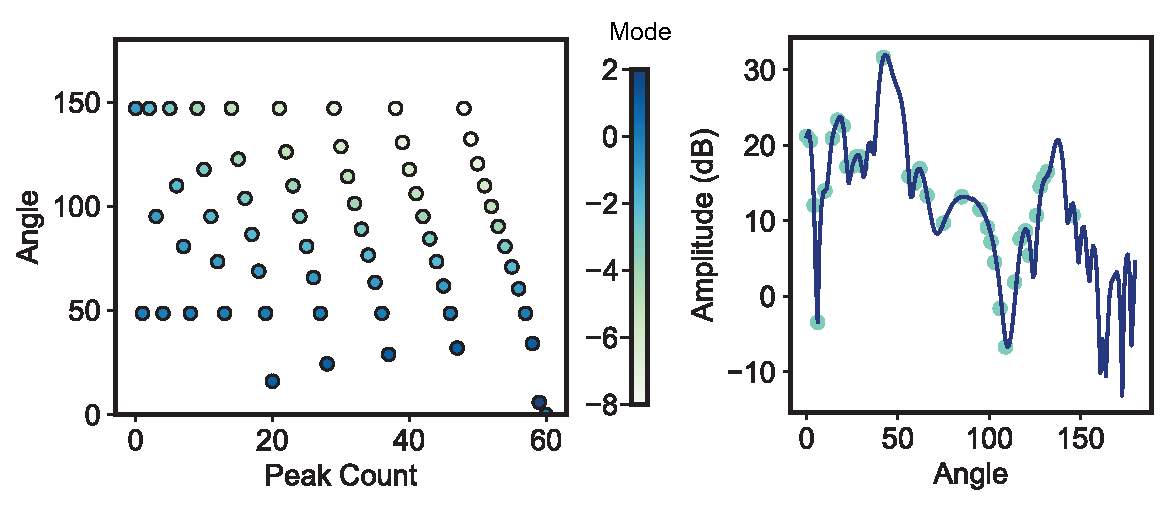
\includegraphics[width=6in]{figures/fig4_labeled2.eps}
	\caption{The left panel shows the possible Floquet modes from any linear combination of modes predicted by Equation 1; as expected, the positive modes occur in forward scattering (< 90$\deg$) and the negative modes in back-scattering. The right panel shows these predicted Floquet modes overlaid on a sample peak profile generated in COMSOL.}
\end{figure}


\noindent To generate our training data, we build a model of a leaky-wave antenna in COMSOL Multiphysics with a slot of length 18 mm divided into 36 sub-slots, each of which is 500 microns in length. 18 sub-slots (exactly half) of the slots are randomly chosen as to be transparent (i.e. a scattering boundary layer) whereas the balance remain metallic and thus do not leak radiation. We automate this random geometry generation and simulation using MPh \cite{john_hennig_2022_6312347}, an open-source Python package that enables controlling COMSOL via its API. Basic combinatorics theory tells us that there are over 9 billion possible slot designs that can be generated, indicating the usefulness of deep neural networks in this prediction task given the sheer number of possible outputs; using only a few tens of thousands sets of training data, we can predict an optimal slot design for an arbitrary peak profile. The simulation geometry is shown in Figure 2a below \\


\begin{figure}[H]
	\caption{Simulation geometry (left) and possible peak profiles (right)}
	\begin{subfigure}[b]{0.45\textwidth}
		\centering
		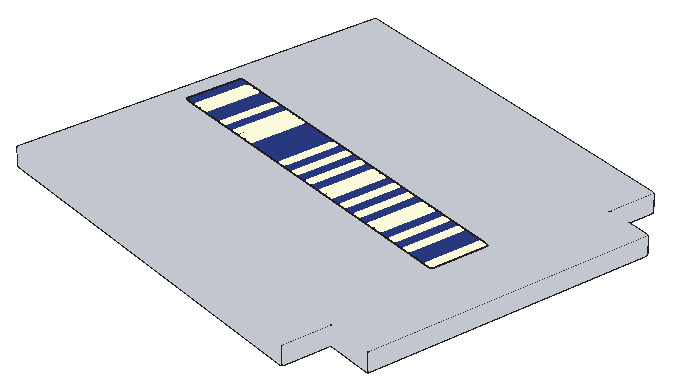
\includegraphics[width = 3.2in]{figures/fig5.eps}
		\caption{The leaky wave antenna geometry used to generate training data. Dark-colored sub-slots represent transparent areas while light colors indicate metallic boundaries; both are randomly generated so that the slots are half and half.}
	\end{subfigure}
	\begin{subfigure}[b]{0.55\textwidth}
		\centering
		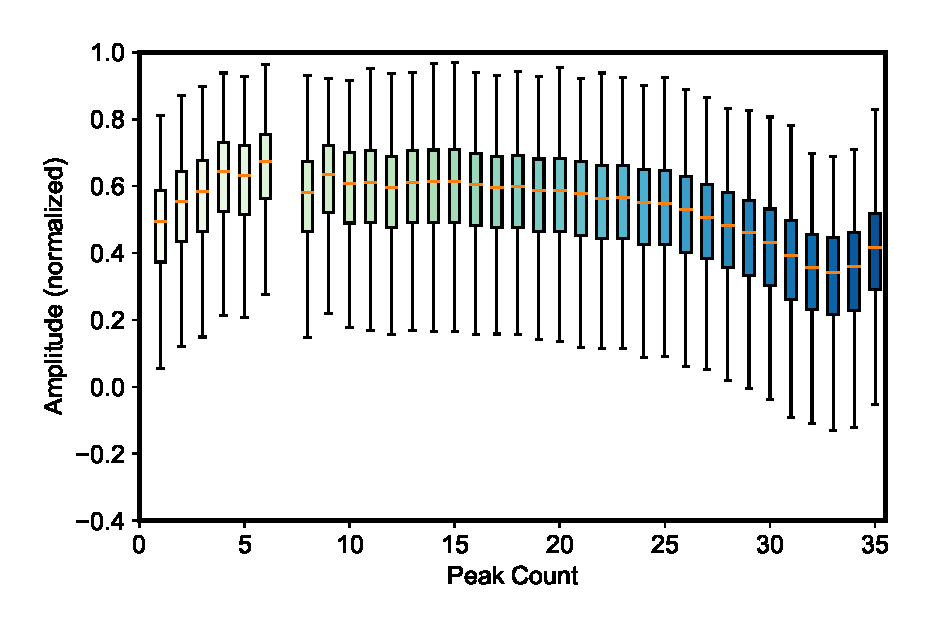
\includegraphics[width=3in]{figures/fig2new.eps}

		\caption{A box plot showing the amplitudes at each peak; peak \#23 is always the highest amplitude because it is the primary emission angle of all LWAs, periodic and not, at 200 GHz. A wide array of values are evident.}
	\end{subfigure}

\end{figure}


\noindent 25,000 instances of COMSOL simulation data is used as the data source for our deep neural network, with a test-train split of 80-20. Figure 2b above shows the possible values for each peak, giving an approximate range over which we can design peak profiles for this particular geometry. The network, which is built with TensorFlow, has six dense layers, each of which have 2000 neurons and use a LeakyReLU activation function with $\alpha = 0.1$. The model uses the Adam optimizer and has a learning rate of 0.0001 and predicts the output of each individual sub-slot with a sigmoid activation function indicating the probability that a given sub-slot should be transparent. The model architecture is visualized in Figure 3. \\

\begin{figure}[b]
	\centering
	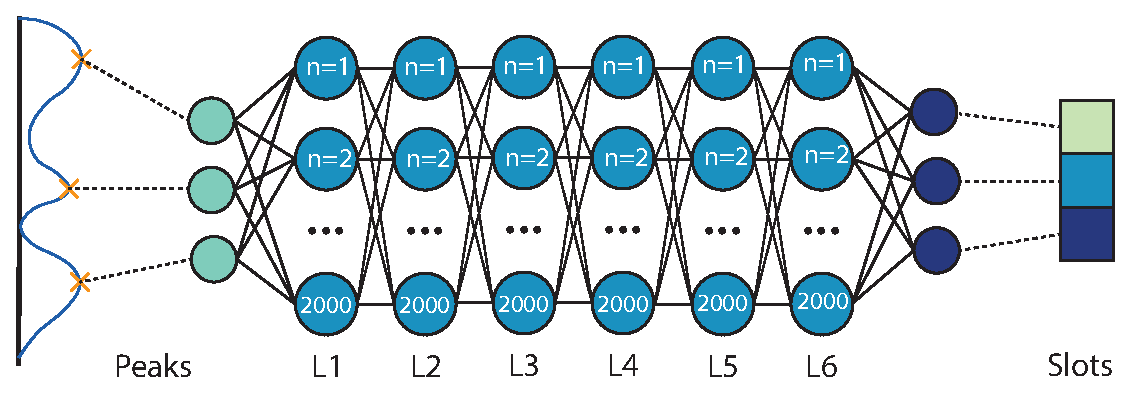
\includegraphics[width=6in]{figures/fig1.eps}
	\caption{Neural network architecture schematic; peaks are used as the input data and passed through six hidden layers to predict the ideal slot design that will yield the closest possible signal.}
\end{figure}

\noindent The tricky part of the inverse problem, as we consider here, is finding an appropriate loss function -- the primary objective is to generate a slot that minimizes the difference in signal compared to what is desired, but in order to use this idea as our loss function, we would need to compute the far-field signal for each slot we generate as we train the model, which would be extraordinary (and unfeasibly) computationally expensive. Thus, instead, we turn to the idea of making the generated slot look as similar to the given training slot for a given peak profile as possible. Given that this is essentially a binary classification problem for each sub-slot, we use three weighted binary cross-entropy (BCE) loss functions, which are summed together to form our overall loss function with the following weightings:
\begin{enumerate}
  \item BCE between the true and predicted slot (2x)
  \item BCE between the first derivative of the true and predicted slot using a Prewitt filter (1x)
  \item BCE between the second derivative of the true and predicted slot using a Laplacian filter (1x)
\end{enumerate}

\section*{Results and Discussion}
\subsection*{Binary Predictions}
For some given peak geometry, the model returns each individual sub-slot's probability of being transparent (i.e. a value close to 0 indicates the sub-slot should be metal, whereas a value close to 1 indicates a transparent sub-slot) using a sigmoid activation function. In Figure 4 below, for two sample peak profiles, the true slots (left), predicted slot (center) and rounded ML slot (right, i.e. making the 16 slots with the highest probabilities transparent and vice versa). Both of these predicted slots share many similarities with the true slot but there are also some differences -- the testing accuracy was about 68\% averaged over all of the training samples. 

\begin{figure}[H]
	\centering
	\subfloat{{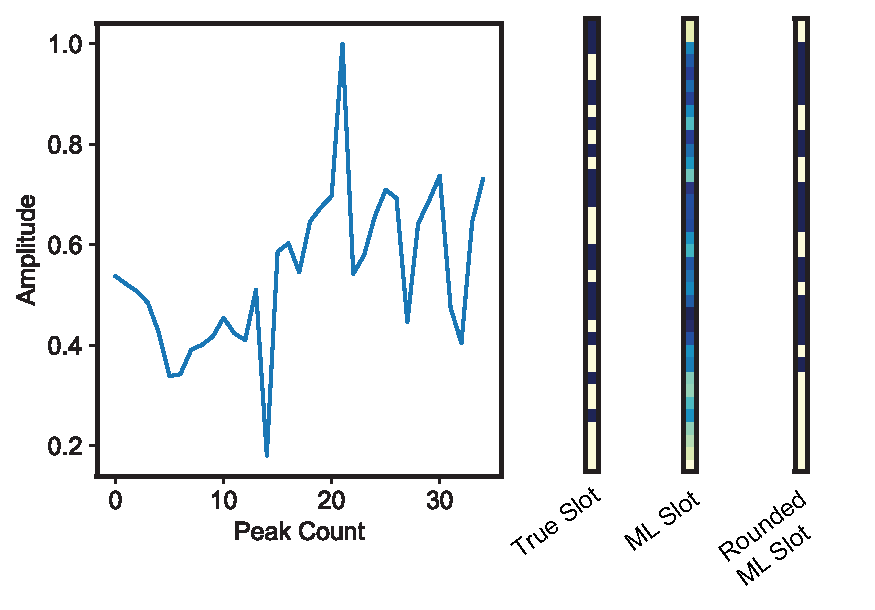
\includegraphics[height=2in]{figures/fig3_labeled.eps}}}
	\subfloat{{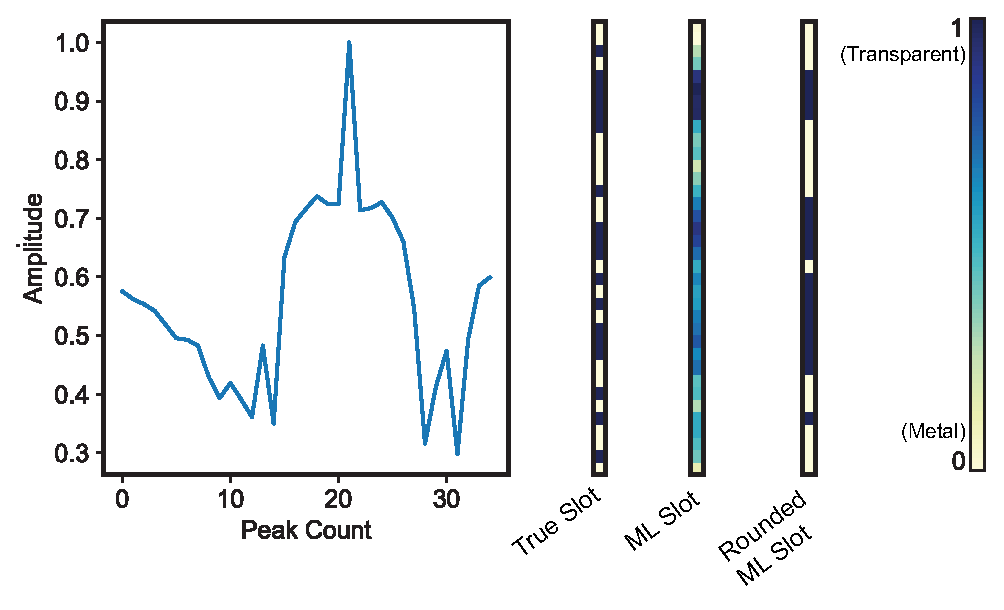
\includegraphics[height=2in]{figures/fig3b_labeled.eps}}}
	\caption{Model predictions for two different peak profiles. The left-most slot design is the randomly generated slot used to generate this profile, the center plot shows the sigmoid probabilities of a transparent sub-slot, and the right-most plot shows the top 16 sub-slots from the probabilities.}
\end{figure}

\noindent However, what determines the usefulness of our model is not the similarity of the slot but the similarity of the signal it generates to the objective. In order to consider the accuracy and usefulness of our model, we extract the predicted slot geometries, choose the top 16 slots based on the probabilities, and pass 500 of these new generated slots into our COMSOL model in order to compare the signal from the ML-generated slot to the originally desired peak profile. We then compare the peak profiles to the objective signal and calculate using the mean square error (MSE), as shown in the top left panel of Figure 5 below; the shape of the distribution matches that of similar work \cite{Nadell:19}. In the other panels of Figure 2, we plot the objective peak profile in black against the peak profile of an ML-generated slot, where the color corresponds to the four colored buckets depicted in the histogram. Overall, the agreement is quite excellent, particularly for the first two buckets (green and light blue), which compose about 60\% of testing samples with trends and relative amplitudes of the peaks agreeing very well. Even in the lower-tiered buckets, like in the bottom right panel of Figure 2, many of the peak profile trends are well matched -- however, there are some areas where the model does not perform as well, resulting in a higher MSE. Overall, though, the agreement is excellent and shows that the model can be used to design an acceptable slot for many potentially desired peak profiles. 


\begin{figure}[H]
	\centering
	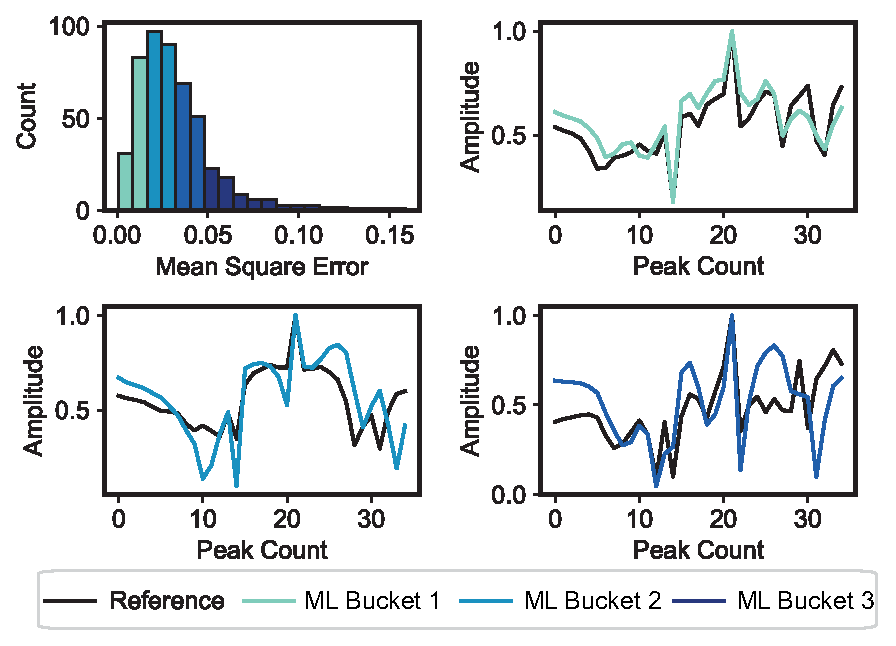
\includegraphics{figures/fig2_labeled.eps}
	\caption{Results from COMSOL simulations of ML-generated slots. The top left panel shows an MSE histogram while the others compare the ML-slot generated peak profile to the objective.}
\end{figure}




\section*{Conclusion}

\bibliographystyle{plain}
\bibliography{references.bib}
\end{document}
